% Copyright 2004 by Till Tantau <tantau@users.sourceforge.net>.
%
% In principle, this file can be redistributed and/or modified under
% the terms of the GNU Public License, version 2.
%
% However, this file is supposed to be a template to be modified
% for your own needs. For this reason, if you use this file as a
% template and not specifically distribute it as part of a another
% package/program, I grant the extra permission to freely copy and
% modify this file as you see fit and even to delete this copyright
% notice. 

\documentclass{beamer}
\usepackage{graphics,epsfig,graphicx,float,subfigure,color}

% There are many different themes available for Beamer. A comprehensive
% list with examples is given here:
% http://deic.uab.es/~iblanes/beamer_gallery/index_by_theme.html
% You can uncomment the themes below if you would like to use a different
% one:
%\usetheme{AnnArbor}
%\usetheme{Antibes}
%\usetheme{Bergen}
%\usetheme{Berkeley}
%\usetheme{Berlin}
%\usetheme{Boadilla}
%\usetheme{boxes}
%\usetheme{CambridgeUS}
%\usetheme{Copenhagen}
%\usetheme{Darmstadt}
\usetheme{default}
%\usetheme{Frankfurt}
%\usetheme{Goettingen}
%\usetheme{Hannover}
%\usetheme{Ilmenau}
%\usetheme{JuanLesPins}
%\usetheme{Luebeck}
%\usetheme{Madrid}
%\usetheme{Malmoe}
%\usetheme{Marburg}
%\usetheme{Montpellier}
%\usetheme{PaloAlto}
%\usetheme{Pittsburgh}
%\usetheme{Rochester}
%\usetheme{Singapore}
%\usetheme{Szeged}
%\usetheme{Warsaw}

\title{Parallel Two-dimensional Fast Fourier Transform}

% A subtitle is optional and this may be deleted
%\subtitle{Optional Subtitle}

%\author{F.~Author\inst{1} \and S.~Another\inst{2}}
\author{Sijing Guo \and Xinyang Wang}
% - Give the names in the same order as the appear in the paper.
% - Use the \inst{?} command only if the authors have different
%   affiliation.

\institute[Courant Institute of Mathematical Sciences] % (optional, but mostly needed)
{
 %\inst{1}%
Courant Institute of Mathematical Sciences
\and Final Project of High Performace Computing}
%  University of Somewhere
%  \and
%  \inst{2}%
%  Department of Theoretical Philosophy\\
%  University of Elsewhere}
% - Use the \inst command only if there are several affiliations.
% - Keep it simple, no one is interested in your street address.

%\date{Conference Name, 2013}
% - Either use conference name or its abbreviation.
% - Not really informative to the audience, more for people (including
%   yourself) who are reading the slides online

%\subject{Theoretical Computer Science}
% This is only inserted into the PDF information catalog. Can be left
% out. 

% If you have a file called "university-logo-filename.xxx", where xxx
% is a graphic format that can be processed by latex or pdflatex,
% resp., then you can add a logo as follows:

% \pgfdeclareimage[height=0.5cm]{university-logo}{university-logo-filename}
% \logo{\pgfuseimage{university-logo}}

% Delete this, if you do not want the table of contents to pop up at
% the beginning of each subsection:
%\AtBeginSubsection[]
%{
% \begin{frame}<beamer>{Outline}
%   \tableofcontents[currentsection,currentsubsection]
%  \end{frame}
%}

% Let's get started
\begin{document}

\begin{frame}
  \titlepage
\end{frame}

%\begin{frame}{Outline}
 % \tableofcontents
  % You might wish to add the option [pausesections]
%\end{frame}

% Section and subsections will appear in the presentation overview
% and table of contents.

\section{1D FFT}
\begin{frame}{1D FFT}
\begin{figure}
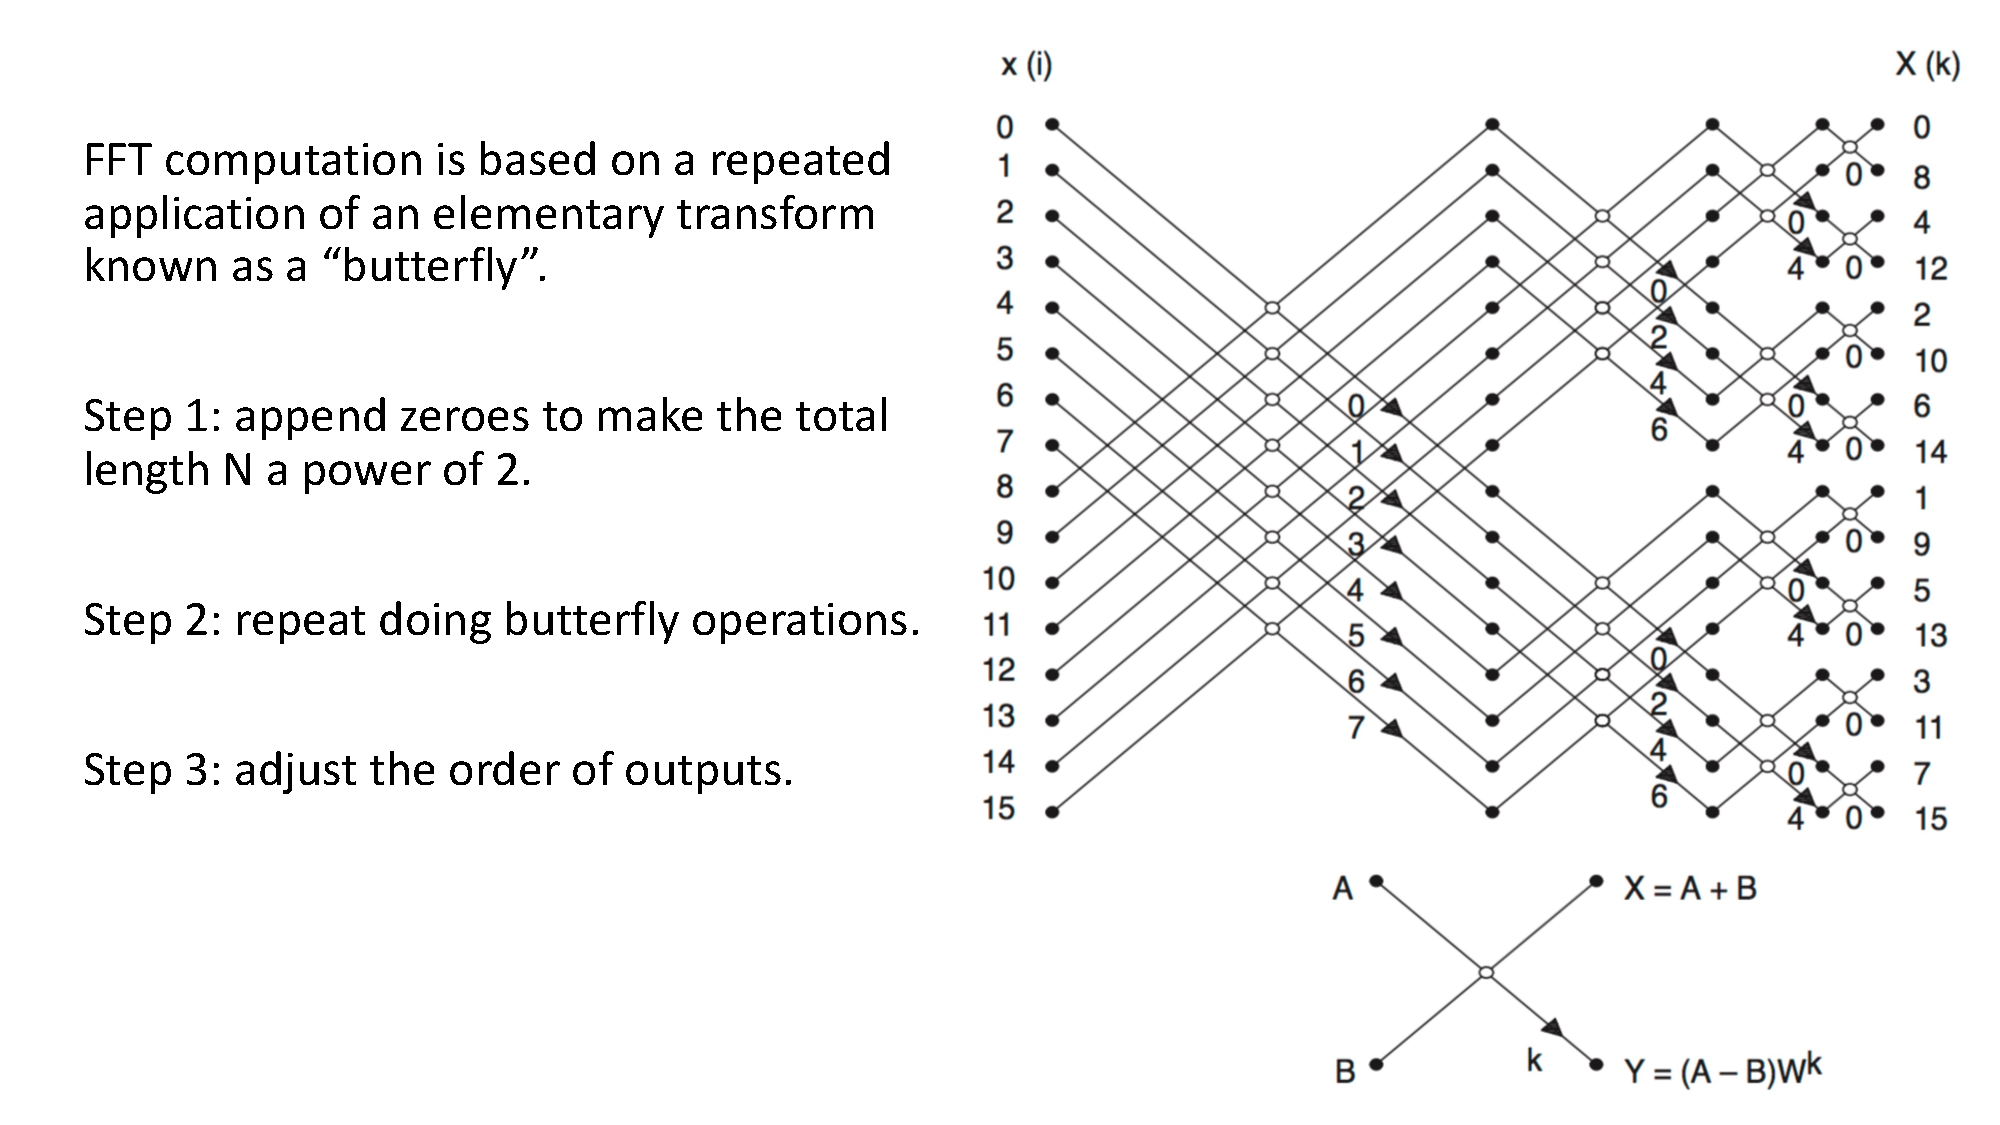
\includegraphics[width=\linewidth]{butterfly.pdf}
\end{figure}
Fastest Fourier Transform in the West (FFTW) is known as the fastest free software implementation of the FFT algorithm. It supports a variety of algorithms and chooses the one it estimates to be preferable in the particular circumstances. 
\end{frame}

\section{Sequential 2D FFT}

%\subsection{First Subsection}

\begin{frame}{Sequential 2D Discrete Fourier Transform (DFT)}
Suppose the 2D signals are stored in a $N_1\times N_2$ matrix $\textbf{x}$. The 2D DFT of $\textbf{x}$ is defined as 
$$X_{r_1,r_2}=\sum_{l_1=0}^{N_1-1}\sum_{l_2=0}^{N_2-1}x_{l_1,l_2}\exp({-\frac{2\pi i}{N_1}r_1l_1})\exp({-\frac{2\pi i}{N_2}r_2l_2})$$
$$r_1=0,1,\cdots, N_1-1 \text{, and } r_2=0,1,\cdots,N_2-1$$
Total computational cost: $O(N_1^2N_2^2)$.\\
\vspace{0.5cm}
This can be reduced significantly by separating the 2D-DFT into a series of 1D-DFTs, which can each be implemented using a fast 1D-FFT algorithm.
\end{frame}

\subsection{Second Subsection}

% You can reveal the parts of a slide one at a time
% with the \pause command:
\begin{frame}{Sequential 2D FFT}
\vspace{-1cm}
\begin{align*}
X_{r_1,r_2}&=\sum_{l_1=0}^{N_1-1}\sum_{l_2=0}^{N_2-1}x_{l_1,l_2}\exp({-\frac{2\pi i}{N_1}r_1l_1})\exp({-\frac{2\pi i}{N_2}r_2l_2})\\
&=\sum_{l_1=0}^{N_1-1}\exp({-\frac{2\pi i}{N_1}r_1l_1})\left(\sum_{l_2=0}^{N_2-1}x_{l_1,l_2}\exp({-\frac{2\pi i}{N_2}r_2l_2})\right)\\
&= \sum_{l_1=0}^{N_1-1}\exp({-\frac{2\pi i}{N_1}r_1l_1})\tilde{X}_{l_1,r_2}\\
&=\sum_{l_1=0}^{N_1-1}\tilde{X}_{l_1,r_2}\exp({-\frac{2\pi i}{N_1}r_1l_1})
\end{align*}
Do 1D FFTs on the $N_1$ rows (of length $N_2$), and then do 1D FFT2 on the $N_2$ columns (of length $N_1$). Total computational cost is  $O(N_1N_2log_2(N_1N_2))$.
\end{frame}

\begin{frame}{Row-Column Method}
\begin{itemize}
\item Step 1: 1D FFTs on the rows (locally).
\item Step 2: matrix transpose.
\item Step 3: 1D FFTs on the rows again (locally).
\item Step 4: matix transpose.
\end{itemize}
\begin{figure}
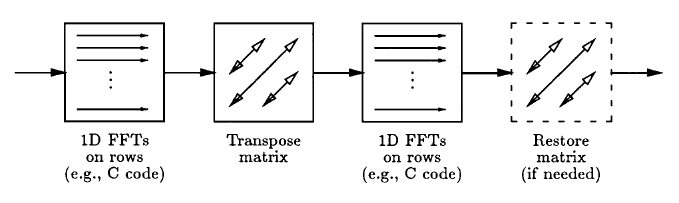
\includegraphics[width=\linewidth]{fft1.png}
\end{figure}
\end{frame}

\begin{frame}{Parallel 2D FFT}
\begin{itemize}
\item 1D FFT can be computed locally. Use FFTW library to do the 1D FFT.
\item Communication is only needed during the transpose step (hardest).
Imagine there are blocks in each processor and use MPI Alltoall 	function to exchange blocks of data with every other processor. Then do the transpose for each block of data.
\end{itemize}
\begin{figure}
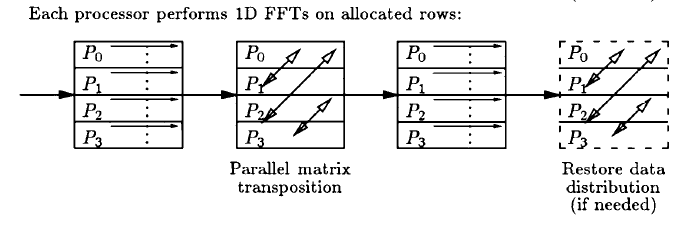
\includegraphics[width=\linewidth]{fft2.png}
\end{figure}
\vspace{-1cm}
\begin{figure}
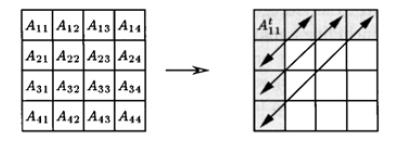
\includegraphics[width=0.6\linewidth]{transpose.png}
\end{figure}
\end{frame}

\begin{frame}{Scalability}
\begin{itemize}
\item Strong scalability: square matrix N=8192, number of processors: $2^{j}$, $j=0,\cdots,10$. 
\item Weak scalability: keep the number of data in each processor fixed $512\times512$.
\end{itemize}
\begin{figure}
	\subfigure[Strong scalability]{
		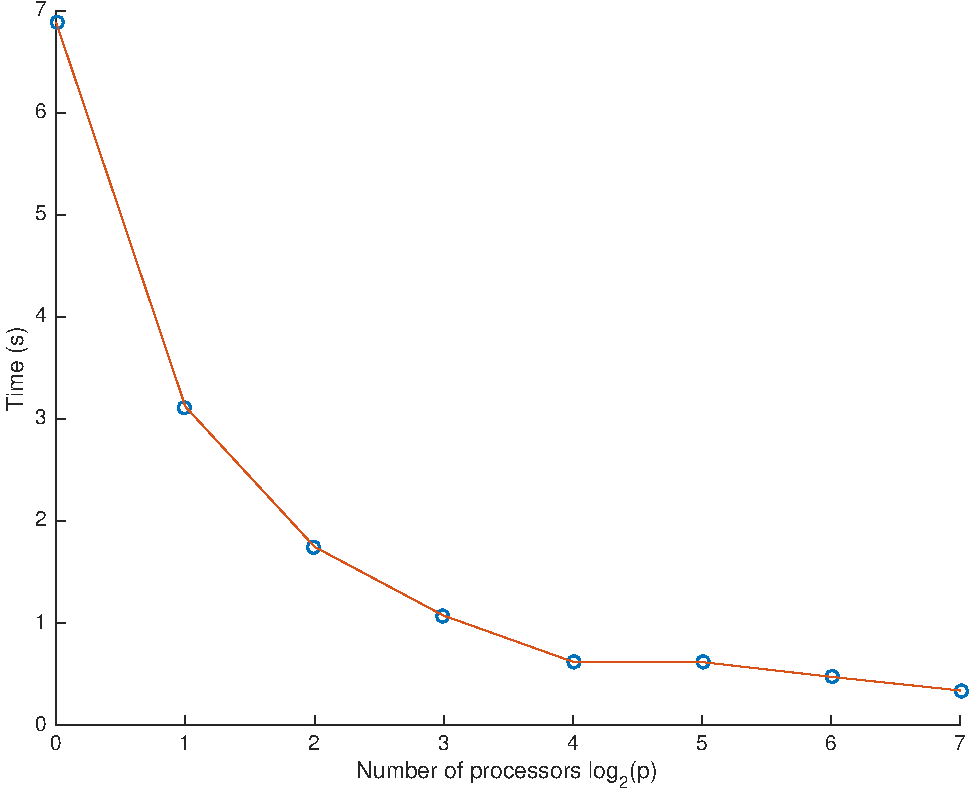
\includegraphics[width=0.48\linewidth, height=5cm]{strong-crop.pdf}}
	\subfigure[Weak scalability]{
		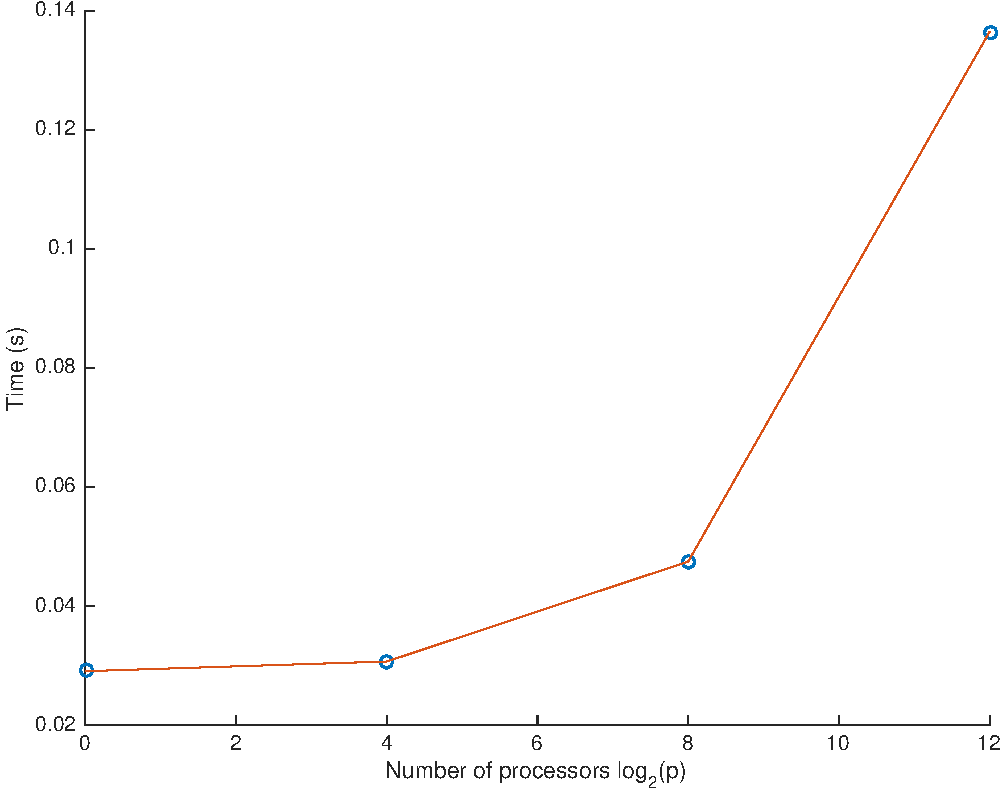
\includegraphics[width=0.48\linewidth, height=5cm]{weak-crop.pdf}}
%	\caption{}
\end{figure}
\end{frame}

\begin{frame}
\begin{itemize}
\item Strong and weak scalability are clear when p is small. 
\item Communication in the transpose step dominates when p is large.
\item When p is too large, running time may increase.
\item 2D version FFTW takes 10s to compute this problem when N=8192. Parallel version is much faster.
\item Efficient transpose algorithm is needed to improve the performance.
\end{itemize}
\end{frame}



% All of the following is optional and typically not needed. 
%\appendix
%\section<presentation>*{\appendixname}
%\subsection<presentation>*{For Further Reading}

\begin{frame}[allowframebreaks]
%  \frametitle<presentation>{Reference}
    
  \begin{thebibliography}{10}
    
  \beamertemplatebookbibitems
  % Start with overview books.

  \bibitem{Author1990}
    Chu, Eleanor and Alan George
    \newblock { Inside the FFT black box: serial and parallel fast Fourier transform algorithms.}.
    \newblock \ CRC Press, 1999.
 
    
  \beamertemplatearticlebibitems
  % Followed by interesting articles. Keep the list short. 

  \bibitem{FFTW}
   Matteo Frigo and Steven G. Johnson
    \newblock FFTW Manual
  %  \newblock {\em Journal of This and That}, 2(1):50--100,
 %   2000.
 \bibitem{1DFFT}
 Piedra, Rose Marie. 
 \newblock Parallel 1-D FFT: Implementation with TMS320C4x DSPs. 
 \newblock \ Texas Instruments, 1992.
  \end{thebibliography}
\end{frame}

\end{document}


